\section{Requisitos}
\label{sec:requisitos}
\subsection{Requisitos Funcionais}

\begin{itemize}
\item Armazenar garrafas recicláveis.
\item Bonificar usuário por entrega de garrafas.
\item Armazenamento separado pelos tipos de materiais de garrafas.
\item Triturar as garrafas de plástico.
\item Validar o tipo de objeto a ser inserido na máquina.
\item A alimentação energética será diretamente pela rede elétrica.
\item Deverá haver a interação de reconhecimento direto entre máquina e usuário.
\item Manter dados do usuário.
\item Projeto de estrutura que comporte aparatos tecnológicos.
\item Projeto de estrutura que comporte o motor, o separador, triturador e compartimentos de armazenagem.

\end{itemize}

\subsection{Requisitos Não Funcionais}

\begin{itemize}
\item Haverá sistema de segurança de desligamento do motor.
\item Armazenar as garrafas de vidro de forma intacta.
\item O sistema da máquina deve guardar os dados em um banco em nuvem.
\item A máquina deve atender à normas legais.
\item A máquina terá seu uso liberado após a identificação do usuário.
\item Não deve ser exposto nenhum dado privado do usuário de forma livre.
\item A estrutura do triturador deve ser extremamente fechado a qualquer contato do usuário. 

\end{itemize}

\section{Estudo da Viabilidade do Projeto}

\subsection{Infra-estrutura}
    O espaço disponível para desenvolvimento do projeto é o Galpão da FGA, o qual nos fornece um série de ferramentas que serão úteis para para a produção da estrutura da máquina.

\subsection{Viabilidade técnica}
    O projeto consiste em uma máquina que irá receber uma garrafa, separá-la com base no seu tipo, podendo ser plástico ou vidro, e triturando-a caso a mesma seja de plástico. A estrutura principal, responsável por suportar os componentes dos subsistemas(e.g. triturador), será construída com materiais acessíveis e de baixo custo, visando a construção de um protótipo que garanta a integridade dos subsistemas. O triturador será ornamentado com base em projetos open source já construídos e testados\cite{preciousplastic}. O seletor será implementado com componentes já utilizados em máquinas como as fresadoras CNC, sendo portanto um mecanismo já muito estudado e com muito material fonte para consulta \cite{hacksterDamian} e \cite{hacksterArduino}.

\subsection{Gestão e Pessoal}
    Os alunos responsávei por desenvolver o projeto são todos de Engenharias (Aeroespacial, Automotiva, Eletrônica, Energia e Software), com o apoio de professores de alto gabarito no que diz respeito à gerência de projeto e à condução da disciplina de Projeto Integrador de Engenharia II. Além disso, durante o semestre serão conduzidos pontos de controle para que seja realizado um acompanhamento do projeto, afim de garantir que, apesar de eventuais problemas, todos os sistemas serão entregues.

\subsection{Planejamento estratégico}

\begin{figure}[!ht]
	\centering
		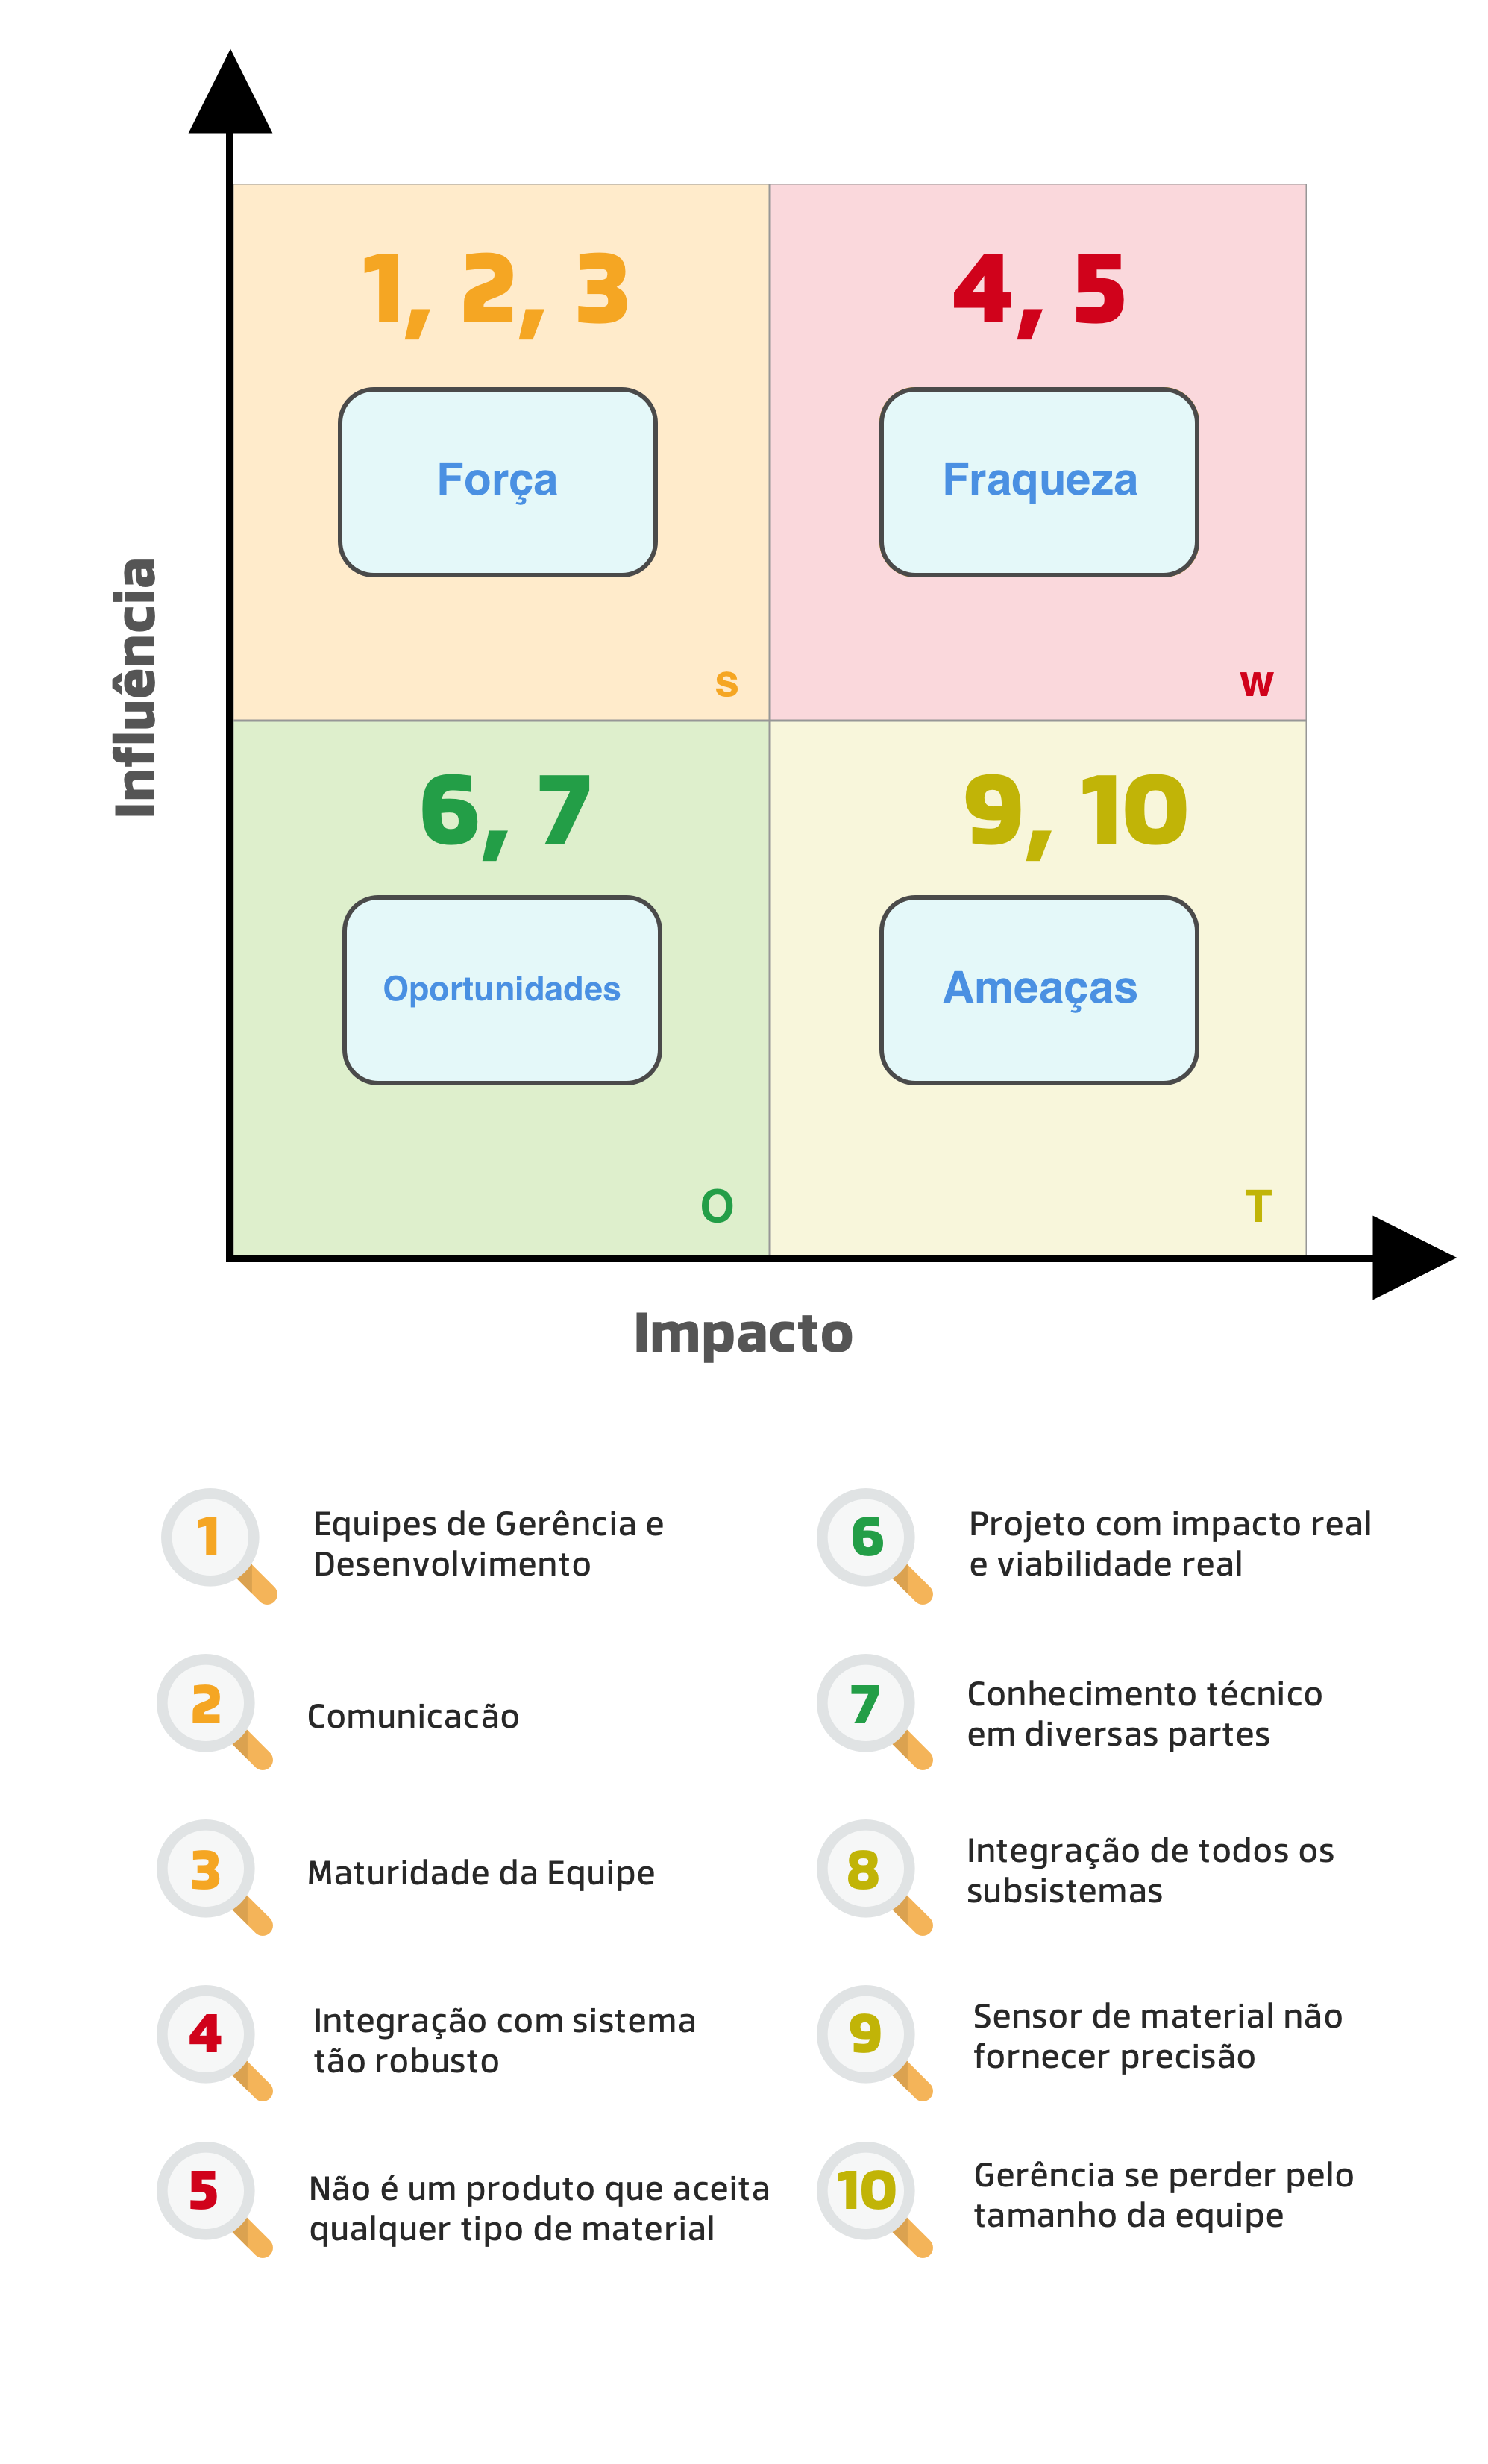
\includegraphics[scale=0.1]{figuras/swot}
	\caption{Matriz SWOT.}
\end{figure}

\subsubsection{Forças(S)}
Equipes de Gerência de Desenvolvimento:

    A equipe de gerência conseguiu se adequar da melhor forma para gerenciar toda a equipe que não se conhecia. Vários membros se mostram aptos no que se refere ao conhecimento técnico.

Comunicação:

    Logo no início do projeto, a equipe se comunicou com excelência. Foi escolhido as ferramentas apropriadas para as atividades da primeira entrega, onde todos os integrantes estavam presentes e cientes.

Maturidade da Equipe:

    A equipe de mostra muito madura em tomada de decisões. Cada subsistema se mostra com qualidade de agregar valor ao que for necessário, e vários membros se mostram ativos no mercado e em práticas gerais necessárias para o projeto. 


\subsubsection{Fraquezas(W)}
Integração com sistema tão robusto:

    Os integrantes de cada subsistema não estão acostumados em integrar com outras áreas, sendo um obstáculo a ser batido ao longo do projeto.

Não é um produto que aceita qualquer tipo de material:

    Esse limitação inviabiliza trabalhar com qualquer tipo de garrafa.


\subsubsection{Oportunidades(O)}
Projeto com impacto real e viabilidade real:

    O projeto em questão tem real impacto e viabilidade na comunidade, sendo motivador trabalhar com tal projeto.

Conhecimento técnico em diversas partes:

    Devido a todos os obstáculos necessários vencer, o potencial de conhecimento técnico adquirido é de extremo valor e importância.

\subsubsection{Ameaças(T)}
Integração de todos os subsistemas:
    
    Subsistemas separados podem funcionar da melhor forma, mas sem integração o projeto se torna inviável. Tempo e conhecimento técnico são ameaças para essa integração.

Sensor de Material não fornecer precisão:

    Qualidade do sensor comprado não fornecer exatamente o que foi planejado para separação das garrafas.


\section{Escopo}
\subsection{Definição do Escopo}
    A proposta do projeto consiste em um sistema de recompensas por meio da reciclagem de garrafas vazias, as mesmas podendo ser de plástico ou de vidro.

    A estrutura básica é composta por uma máquina onde o usuário poderá inserir garrafas PET transparentes de até 600ml ou garrafas de vidro de até 355ml; esta limitação é melhor explicada na seção de subsistemas. Uma vez que a garrafa é inserida na máquina, caso a mesma seja de plástico, ela deverá ser triturada e armazenada em um recipiente dedicado às garrafas de plástico. Caso contrário, a garrafa deverá ser armazenada em um recipiente dedicado às garrafas de vidro. Além disso, a máquina analisará se a garrafa inserida é valida ou não de acordo com os parâmetros definidos neste escopo, por meio de um mecanismo de pesagem e seleção.

    O triturador de plástico será movido por um motor elétrico, o qual estará protegido contra possíveis irregularidas através de um relé térmico. 

    Além disso, o sistema contará com um processo de interação com o usuário através de um aplicativo. O mesmo precisará se identificar por meio de um QR Code vinculado à sua conta, e que será lido pela máquina. O aplicativo também disponibilizará quanto o usuário já acumulou no sistema de recompensa. Haverá também um servidor dedicado a fazer a conexão entre o aplicativo e a máquina.

    Não obstante, a máquina também tomará parte na interação com o usuário, mostrando informações relevantes em um display LCD e emitindo confirmações sonoras através de um buzzer.

\subsection{Processo de Formalização de Aprovação}
    Este processo tem por objetivo regular todas as entregas feitas durante o desenvolvimento do sistema.

    Segue o processo e suas respectivas atividades descritas.

\begin{figure}[!ht]
	\centering
		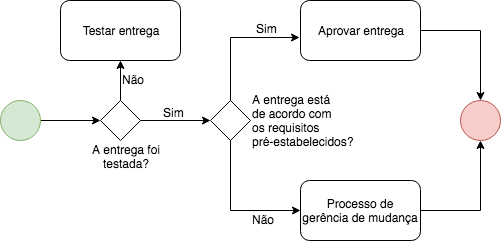
\includegraphics[scale=0.7]{figuras/entrega}
	\caption{Processo de Gerenciamento de Mudança.}
\end{figure}

\begin{itemize}
    \item \textbf{Testar entrega}
        Nesta atividade, deve-se garantir que o que foi desenvolvido está pronto para uso e integração com o resto do sistema, bem como se não apresenta falhas na possibilidade de uso extremo do que foi desenvolvido.

    \item \textbf{Processo de Gerenciamento de Mudança}
        Caso o que foi desenvolvido não esteja de acordo com o que foi previamente acordado nos requisitos do projeto, descritos no começo dessa seção, a mudança deve ser passada por um Processo de Gerenciamento de Mudança antes que possa ser aprovado. O processo em si é melhor descrito na próxima seção.

    \item \textbf{Aprovar entrega}
        Uma vez que a entrega está testada e de acordo com os requisitos do projeto ela pode ser dita como entregue.
\end{itemize}

\subsection{Processo de Gerenciamento de Mudança}
    Sempre que for necessário que mudanças ocorram dentro do sistema, primeiro deve ser executado um processo de gerenciamento de mudança para garantir que a mesma não terá um impacto negativo sobre o projeto.

\begin{figure}[!ht]
	\centering
		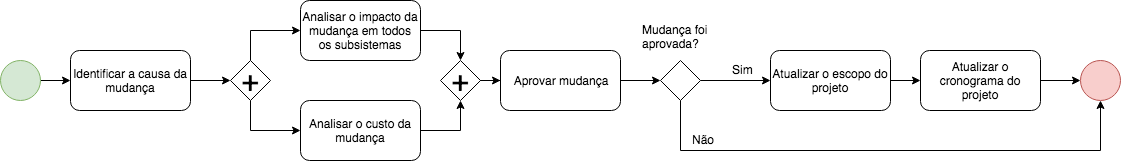
\includegraphics[scale=0.4]{figuras/mudanca}
	\caption{Processo de Gerenciamento de Mudança.}
\end{figure}

    O processo de gerenciamento de mudança envole as seguintes atividades:
\begin{itemize}
    \item \textbf{Identificar a causa da mudança}
        Nesta atividade deve ser identificada a mudança a ser executa e a razão de tal mudança, afim de facilitar as próximas atividades do processo.

    \item \textbf{Analisar o impacto da mudança em todos os subsistemas}
        Uma vez identificada a causa da mudança, a equipe deverá analisar como a mudança irá afetar todos os subsistemas do projeto. Essa atividade deverá resultar na identificação de tudo o que deve ser alterado em cada subsistema, bem como em sua respectiva análise.

    \item \textbf{Analisar o custo da mudança}
        Nesta atividade a equipe deve analisar o custo que a mudança trará ao projeto, tanto a nível financeiro como a nível de tempo restante para desenvolvimento do projeto.

    \item\textbf{Aprovar mudança}
        Com base nas análises de custo e impacto feitas, a equipe deve decidir se a mesma será aprovada caso não haja prejuízo.

    \item \textbf{Atualizar o escopo do projeto}
        Todas as mudanças identificadas na atividade de Analisar o impacto da mudança em todos os subsistemas devem ser incorporadas ao escopo.

    \item \textbf{Atualizar o cronograma do projeto}
        Para que o prazo do projeto seja respeitado, o cronograma deve passar a englobar as mudanças feitas no escopo na atividade previamente descrita.

\end{itemize}

\section{Análise Crítica de Projeto e Desenvolvimento}
    Este tópico se encontra inserido no apêndice no Planejamento de Riscos e Registro de Riscos.

\section{Recursos Humanos}
\subsection{Papéis e responsabilidades}

O projeto de separação de garrafas será desenvolvido e composto por 13 integrantes sendo dividido em 4 equipes, cada uma delas responsável por um subsistema do projeto. Os subsistemas foram definidos para que cada equipe tivesse a possibilidade de trabalhar independentemente, aumentando sua produtividade, e de acordo com o cronograma, integrar os subsistemas em uma fase mais madura do projeto. Os subsistemas definidos para o projeto são:

\begin{itemize}
\item Eletrônica
\item Energia, 
\item Estrutura
\item Software
\end{itemize}

Para cada equipe foi designado um subgerente responsável por supervisionar e coordenar cada subsistema do projeto. A estrutura geral de gerenciamento do projeto pode ser observada na imagem abaixo.

\subsection{Organograma}

\begin{figure}[!ht]
	\centering
		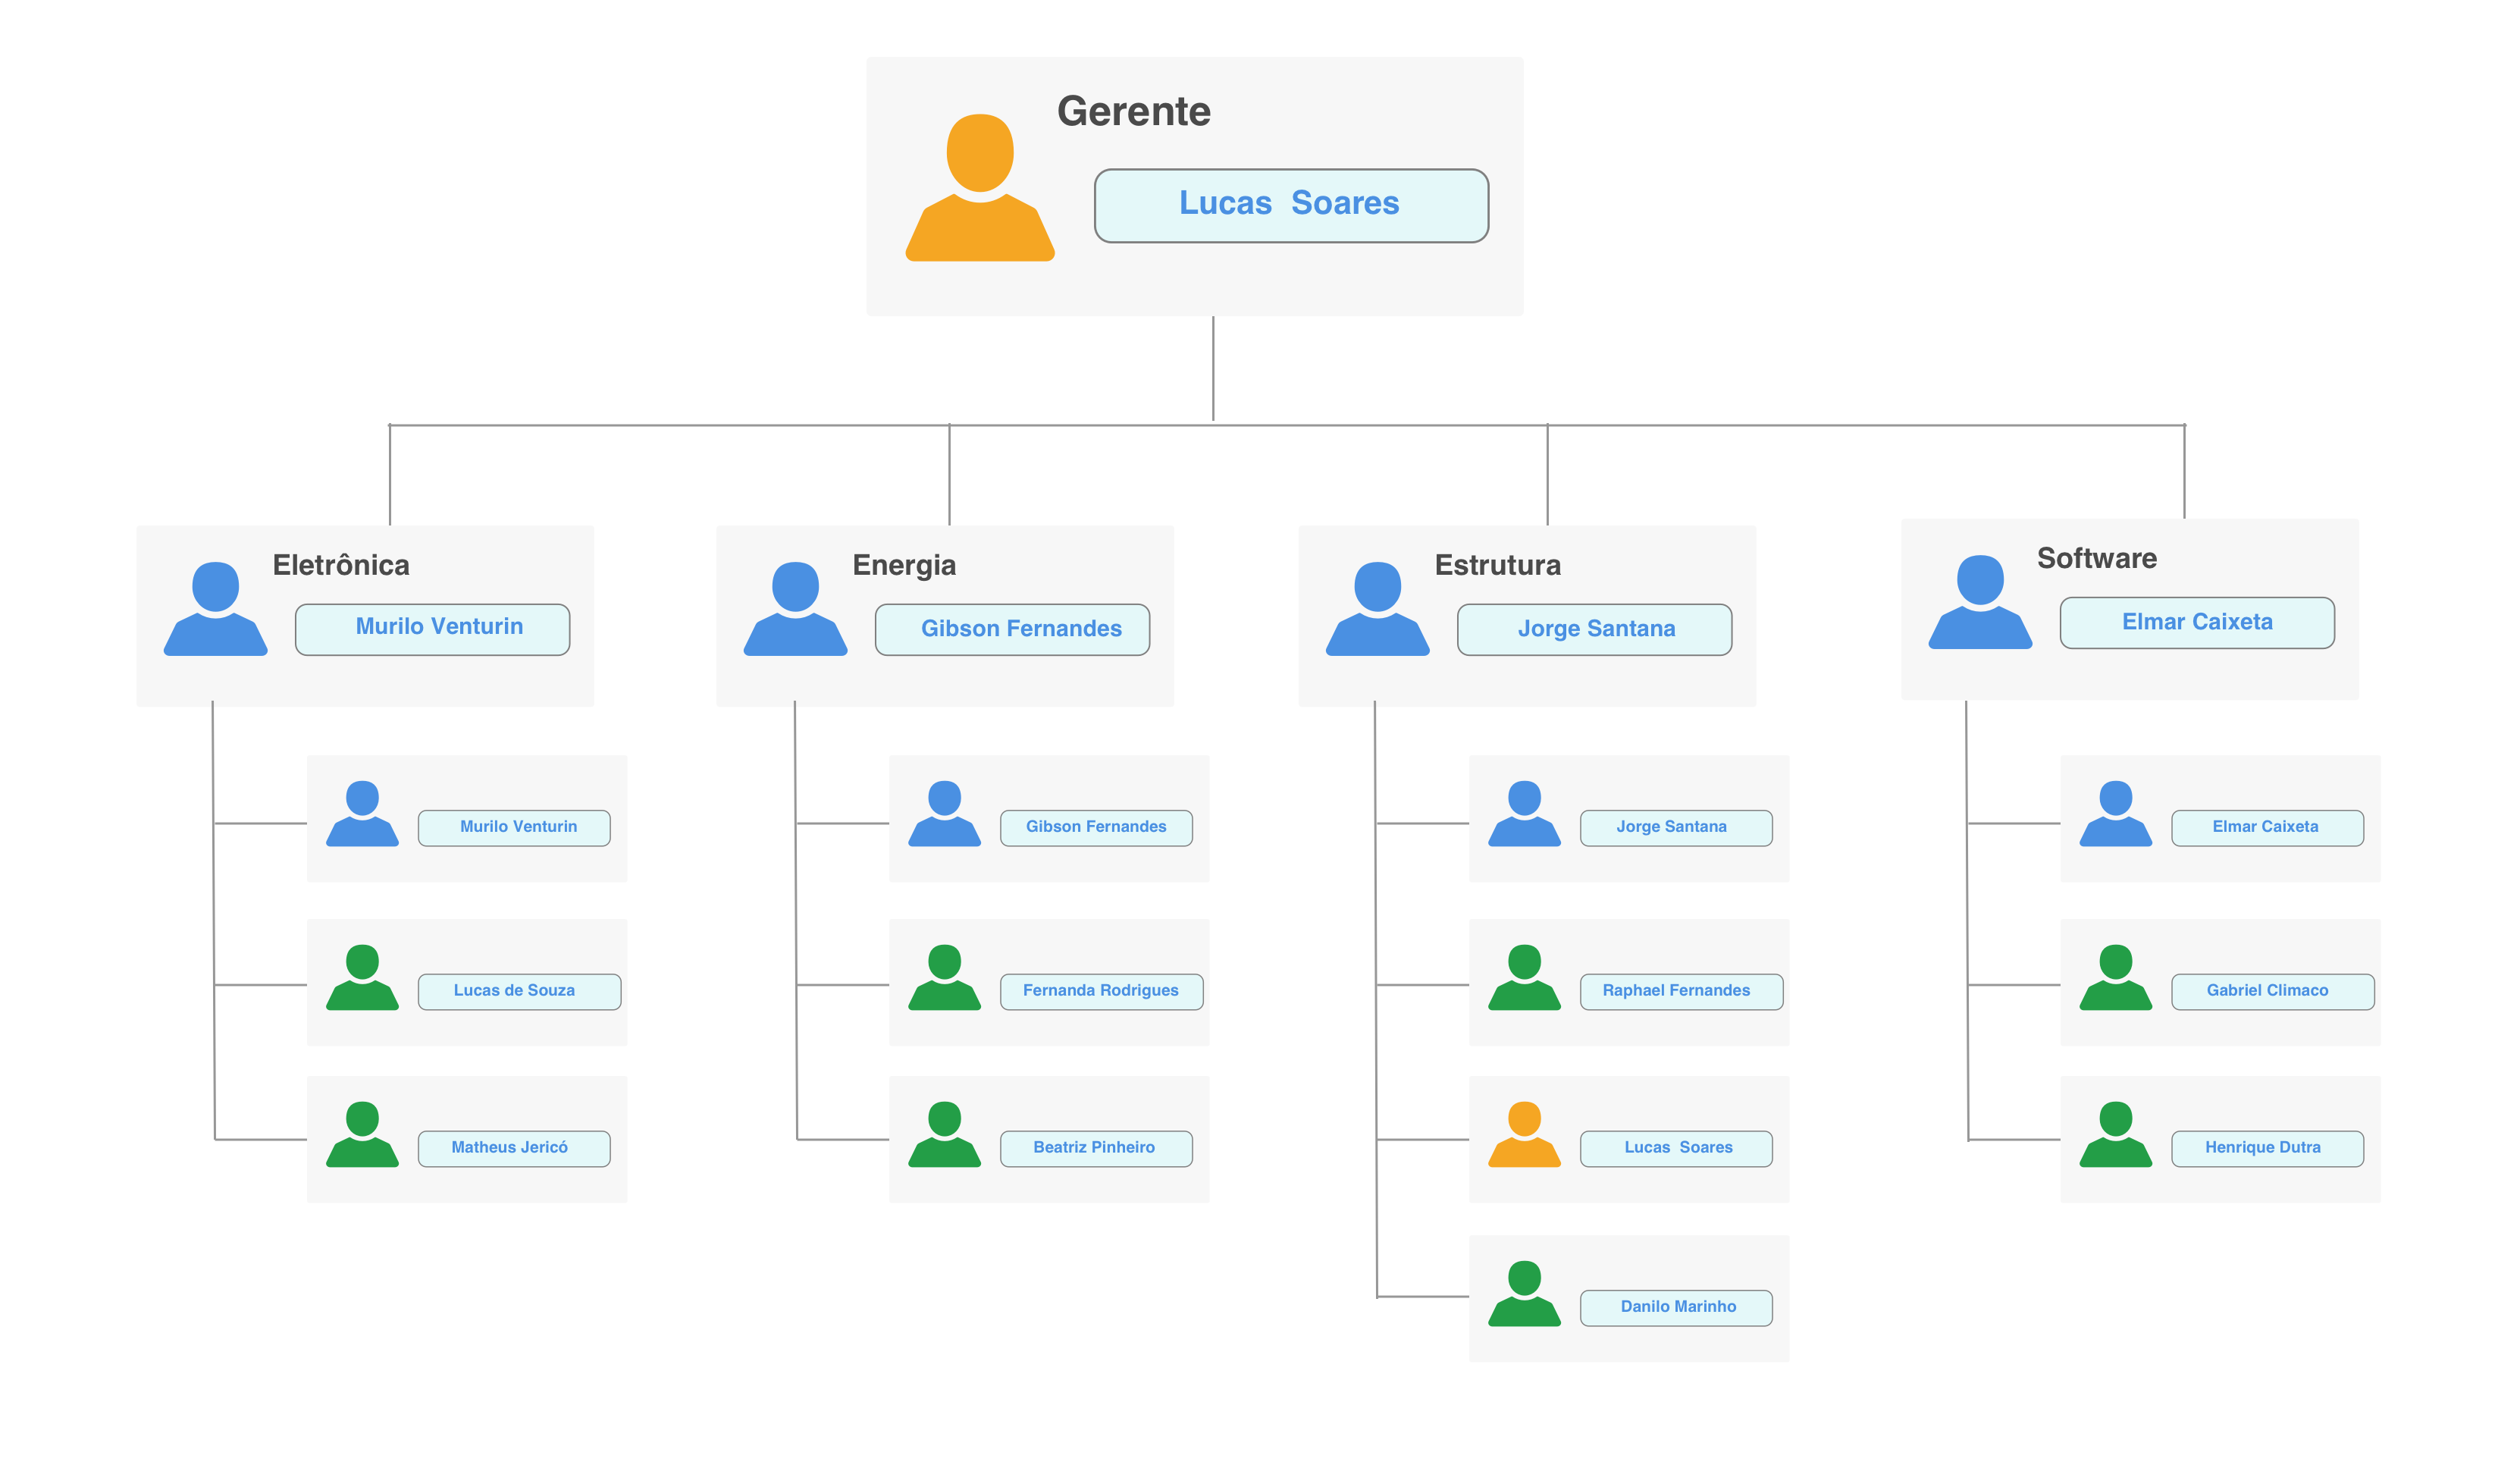
\includegraphics[scale=0.1]{figuras/organograma}
	\caption{Organograma dos papeis do projeto.}
\end{figure}
